\documentclass[11pt,a4paper]{ivoa}
\input tthdefs

\title{Data Origin in the VO}

% see ivoatexDoc for what group names to use here
\ivoagroup{DCP}

%\author[????URL????]{G.Landais}
\author{G.Landais}
\author{G.Muench}
\author{looking for contributors}
%\author{????Fred Offline????}

\editor{G.Landais}

% \previousversion[????URL????]{????Concise Document Label????}
\previousversion{This is the first public release}
       

\begin{document}
\begin{abstract}
The goal of the document is to make the Data Origin more visible in the query results executed in the Virtual Observatory. 
The document lists meta-data required to provide sufficient traceability to end-users in order to improve the understanding 
of the resultsets and enabling its reuse and its citation.

\end{abstract}


\section*{Acknowledgments}

???? Or remove the section header ????

\section*{Conformance-related definitions}

The words ``MUST'', ``SHALL'', ``SHOULD'', ``MAY'', ``RECOMMENDED'', and
``OPTIONAL'' (in upper or lower case) used in this document are to be
interpreted as described in IETF standard RFC2119 \citep{std:RFC2119}.

The \emph{Virtual Observatory (VO)} is a
general term for a collection of federated resources that can be used
to conduct astronomical research, education, and outreach.
The \href{https://www.ivoa.net}{International
Virtual Observatory Alliance (IVOA)} is a global
collaboration of separately funded projects to develop standards and
infrastructure that enable VO applications.


\section{Introduction}

Data origin is required for end users to understand data, for citation and for reusability. The  provenance is cited as a mandatory criterion in the EOSC or in RDA FAIR definition. 

The virtual observatory provides an advanced framework to search and consume data provided by Data Centers or Space Agencies who apply curation in different level.  In this context, Data Origin in output includes meta-data from the data producer (author, space agency) and the Data Center which hosts the resource. 
Depending of the implementation, the users can find the origin information in the Data center web pages (landing pages) or in the Registries of the Virtual Observatory. For citation, the ADS search engine provides citation capabilities offering bibtex. There are no VO standards today to get the information easily. For instance, the origin meta-data are not included neither in output format, nor in protocols used to access the data.
A list of basics meta-data added in strategic location (as result output or resource listing) would give easier the authors search who is looking for how to cite VO resources. Tracing data origin, from the producer to the final query enables also to report to end users the different agents implied in the data preservation (authors, data center, space agencies, journal)- especially when data can be subject to a curation  which depends of the different agents.
We propose to list the meta-data which responds to the need of Provenance and methods available today for their implementations. 

\subsection{Role within the VO Architecture}

%\begin{figure}
%\centering

% As of ivoatex 1.2, the architecture diagram is generated by ivoatex in
% SVG; copy ivoatex/archdiag-full.xml to role_diagram.xml and throw out
% all lines not relevant to your standard.
% Notes don't generally need this.  If you don't copy role_diagram.xml,
% you must remove role_diagram.pdf from SOURCES in the Makefile.

%\includegraphics[width=0.9\textwidth]{role_diagram.pdf}
%\caption{Architecture diagram for this document}
%\label{fig:archdiag}
%\end{figure}

%Fig.~\ref{fig:archdiag} shows the role this document plays within the
%IVOA architecture \citep{2010ivoa.rept.1123A}.

%???? and so on, LaTeX as you know and love it. ????



\section{Use cases}
\begin{itemize}
	\item To get provenance information easier \\
	example: Query the Gaia catalogue using VO services (for instance with topcat or any other VO-software). The registry lists Data Center (eg: Gavo, VizieR, ESA) which provides Gaia  tables using TAP. The results returns VOTable having information in the header. However, the information depends of the implementation.\\
	e.g.:\\
	\begin{itemize}
		\item VizieR, GAVO, ESA provide the ADQL 
		\item GAVO provides the license and ivoid in the output.
		\item ESA provide the license, url to a datalink service
	\end{itemize} 
	To get citation information require the user to query the providers web sites or to use ADS.
	\item Relevant meta-data for final users to cite resources \\
	Provide Data origin output or with API to get all meta-data needed to build bibtex?
	\item Relevant meta-data for final users to understand data origin \\
	Table provided by a Data Center can be a copy of an existing resource. For instance, a table published in a journal or by a Space Agency is also hosted in a Data Center like CDS, GAVO, etc.
	The data curation depends of the Data Center which can add associated data, enrich meta-data (eg: add filter for magnitude) or make a sub-selection of columns.
	\item Give me a bibliography of everything I've used in the workflow", where we'd probably have handwave away "workflow" and say "you can do it per query result  now"
\end{itemize}

The basics meta-data should contain the data origin (space agency or authors, article references), the data center providing the resource, the date of publication ...

\section{State of the art}
Data origins consists in a collection of meta-data that can be consumed by users. Data origin is partially included in Data Models or Data Access Layers. We lists a non exhaustive state of the arts of their usage.

\subsection{Data origin in Data Models}
\subsubsection{ObsCore} 
Obscore is an example which includes in the model Data  identifiers and instruments (mandatory) that can be used to put Data origin. 

\subsubsection{ProvDM}
ProvDM is dedicated for workflows. It is an astronomy extension of the W3C Provenance. The result is a graph which is composed by Entities, Activities and Agents linked together.\\
eg. VizieR workflow can be helpful to get Data Origin:
	
	https://cdsarc.cds.unistra.fr/viz-bin/cat/J/AJ/154/57\\
	https://cdsarc.cds.unistra.fr/viz-bin/provenance?filter=true\&out=prov:png\&cat=J/AJ/154/57 \\
	
	
Note:  a Python library enables to trace the Provenance of a workflow in a graph. It is available for users to trace their python activity (M.Servillat)


\subsection{Data origin in Access layers}

\subsubsection{The registry} 
VO registries,based on OAI-PMH, are harvested by RoR and clients. The registry's schemas allows Data centers to fill data origin in a rich meta-data collection: Identifiers, authors, dates, comments, etc.

List of meta-data useful to trace data origin:
\begin{itemize}
	\item altIdentifier
	\item curation.publisher
	\item curation.creator
	\item date: role= Updated, role=Created
	\item contact
	\item content.subject
	\item content.description
	\item content.source : format=bibcode
	\item content.referenceURL
	\item content.relationship
\end{itemize}


\subsubsection{TAP} 
The TAP protocol includes a schema which describes the tables provided in a service.
The TAP schema doesn't provide any meta-data about origin.


\subsection{Data Origin in VOTable serialization}
DALI proposes the additional information “citation” and "IVOA standard ID" to be in the VOTable header (https://ivoa.net/documents/DALI/20170517/REC-DALI-1.1.html) 

To fill the data origin, each Data Center adopts its own solution :
\begin{itemize}
    \item VizieR catalogues: the first author and the publication year are added in the catalogue title description
    \item Gavo: use the DALI proposal to add ivoid + licences
    \item other example ?
\end{itemize}

Currently in development status, the Mango Data Model is a container used to annotate VOTable. MangoDM uses Mivot  to serialize Data Models instances. This serialization enables links and can include Data Models  in the VOTable header. It could be used to export rich Data Models like Provenance.

\subsection{DOI}
The DOI is a persistent identifier which includes meta-data. We can extract from the Datacite schema as well as the Crossref schema, information which enables to cite the data, to get authors, dates or licenses information.

The richness of information depends on the implementation of the data producers. The information is not homogeneous.

\section{Expected Data Origin}

 \subsection{Link Provenance DM with Data origin}
Translated to Provenance "Entites" and "Agents" are sufficient to establish bibtex – In a full Provenance diagram, Entities can be linked each other with Activities. 
In the Data origin context, we will focus on "Entities" and "Agents".\\ 


\begin{figure}[ht!]
	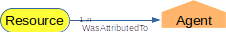
\includegraphics[width=0.5\textwidth]{provenance.png}
	\caption{Entities ans Agent in Provenance schema}\label{provenance}
\end{figure}

Note: Why this limitation ?
Full provenance is adapted to describe workflows. The result is a graph with many branches and its serialization depends of the need of the producers.
The Provenance DataModel is encouraged for any datacenter to describe the workflows  using the serialization adapted for its purpose. To extract from the Provenance model only "Entites" and "Agents" enables homogenization of its usage  and finally simplify the client parsing (no recursivity needed).\\

Note: applied to tables, "Entities" and "Agents" meta-data can by assigned to dataset, collection , table or column and could be serialized into VOTable or TAP schema extension.

\subsection{List of meta-data}
We list meta-data expected to Data origin :

(context: table or dataset resulting from a query)
(in bold, the ProvDM equivalent)

\subsubsection{Agents}
Agents (authors, institutes):  any agents included in the workflow 

\begin{itemize}
    \item Author (\textbf{prov: Agent.type=Person})
    \begin{itemize}
		\item name (\textbf{prov: Agent.name})
		\item Orcid (\textbf{prov: Agent.id})
	\end{itemize}
	\item Institute (\textbf{prov: Agent.type=Organization})
    \begin{itemize}
		\item Name (\textbf{prov: Agent.name})
		\item URL (\textbf{prov: Agent.url})
	\end{itemize}
	\item Data Center (\textbf{prov: Agent.type=Organization})
	\begin{itemize}
		\item Name (\textbf{prov: Agent.name})
		\item URL (\textbf{prov: Agent.url})
	\end{itemize}
	\item Original Data Center (in case of copy/mirror) (\textbf{prov: Agent.type=Organization})
	\begin{itemize}
		\item Name (\textbf{prov: Agent.id})
		\item URL (\textbf{prov: Agent.url})
	\end{itemize}
	\item Editor: journal editor or publisher  (\textbf{prov: Agent.type=Organization})
	\begin{itemize}
		\item name (\textbf{prov: Agent.name})
		\item URL :  Journal web page (\textbf{prov: Agent.url}) 
	\end{itemize}
\end{itemize}

\subsubsection{Resources}
Any resources used to build the result (\textbf{prov: Entity})
\begin{itemize}
	\item Query
	\begin{itemize}
		\item Date of execution (\textbf{prov: Entity.generatedAtTime})
		\item query (adql, ...) (\textbf{prov: Entity.comment})
	\end{itemize}
	\item Table(s) or catalogue(s) (\textbf{prov: Entity})
	\begin{itemize}
		\item Persistent Identifier (\textbf{prov: Entity.id})
		\item VO identifier (ivoid) (\textbf{prov: Entity.?})
		\item URL (landing page) (\textbf{prov: Entity.url})
		\item Date of publication (\textbf{prov: Entity.generatedAtTime})
		\item Curation level (\textbf{prov: ActivityDescription.type or Entity.comment (?)})
		\item Curation activity : simple text – eg: "it is a subset from original data ..." (\textbf{prov: Activity.comment or Entity.comment (?)})
	\end{itemize}
	\item Article(s) (\textbf{prov: Entity})
	\begin{itemize}
		\item Persistent Identifier (\textbf{prov: Entity.id})
		\item Journal name (\textbf{prov: Entity.name})
		\item Date of publication (\textbf{prov: Entity.generatedAtTime})
	\end{itemize}
	\item Any resources completing the original data (\textbf{prov: Entity})
	\begin{itemize}
		\item resource type: filter , computed (\textbf{prov: Entity. ?})\\
		eg: computed column for position, time, etc.
		\item name (\textbf{prov: Entity.name})
		\item comment (\textbf{prov: Entity.comment})
	\end{itemize}
	\item Software used to generate the query (\textbf{prov: Agent=SoftwareAgent})
	\begin{itemize}
		\item user-agent (\textbf{prov:Agent.comment})
	\end{itemize}
	\item Licence (\textbf{prov: Entity})
	\item Copyrights (\textbf{prov: Entity})
\end{itemize}

\section{Implementation tracks}
Several tracks could be explored to provide Data Origin (that we have to define for the context of this document)

\subsection{Data Origin included in VOTable output}
We dress a non exhaustive  list of possible implementation. Tracks using INFO tags are ready-to-client and don't need any development in sofwtare/api.

\begin{itemize}
    \item DOI-based: delegate Data Origin support to DOI and limit the Data origin implemention with adding DOI in <INFO> in the VOTable header
    \item URL-based: delegate citation capability, and other information to specialized services.\\
	The URL could be added in <INFO> in the VOTable headers \\
	Eg: \begin{itemize}
		\item use link to ADS for citation, license, ...
		\item URL to landing page (human readable)
		\item URL to service providing machine-readable output (json/XML)
	\end{itemize}
	\item Semantic-based: define a semantic (mapping with ProvDM could be possible) that can be exploited with <INFO>  in VOTable \\
	e.g.: \begin{itemize}
		\item <INFO name="author" values="name=G. H. Rieke orcid=https://orcid.org/0000-0003-2303-6519"/>
		\item <INFO name="article" value="pid=10.3847/1538-3881/ac3b5d   date=2022  text=The Astronomical Journal, Volume 163, Number 2"/>
		\end{itemize}
	\item MiVOT-based: use Mivot capabilities to add rich Provenance into VOTable header

\end{itemize}

\subsection{Data origin  using dedicated services}
Delegate Data origin capability to services like ADS or VO registries and provides tools/api (for instance in pyVO)  based on ivoid to get the information. 

\subsection{Data origin in Access layer}
Delegate Data origin capability to TAPschema which could describe the Data origin of the tables with table like: $TAP\_SCHEMA.prov\_table$, $TAP\_SCHEMA.prov\_agent$
As the previous case, this track needs to provide api/tools  to get the information and facilitate the usage.


\appendix
\section{Changes from Previous Versions}

No previous versions yet.  
% these would be subsections "Changes from v. WD-..."
% Use itemize environments.


% NOTE: IVOA recommendations must be cited from docrepo rather than ivoabib
% (REC entries there are for legacy documents only)



\bibliography{ivoatex/ivoabib,ivoatex/docrepo}


\end{document}
